\documentclass[tikz,border=10pt]{standalone}
% Shared style for all Speed Demon diagrams: one palette, rounded white boxes,
% dark ink, white page (readable on GitHub light and dark).
\hyphenpenalty=10000 \exhyphenpenalty=10000 \tolerance=9999
\usepackage[T1]{fontenc}
\usepackage[scaled=0.95]{helvet}
\renewcommand{\familydefault}{\sfdefault}
\usepackage{tikz}
\usepackage{pgfplots}
\pgfplotsset{compat=1.16}
\usetikzlibrary{arrows.meta,positioning,shapes.geometric,fit,backgrounds,calc}

\definecolor{ink}{HTML}{1F2937}
\definecolor{mute}{HTML}{6B7280}
\definecolor{rule}{HTML}{9CA3AF}
\definecolor{cA}{HTML}{2563EB}   % Track A  blue
\definecolor{cB}{HTML}{D97706}   % Track B  amber
\definecolor{cC}{HTML}{059669}   % Track C  green
\definecolor{cD}{HTML}{7C3AED}   % Track D  violet
\definecolor{warn}{HTML}{DC2626} % fallback / redo path
\definecolor{wash}{HTML}{F3F4F6}

\tikzset{
  every node/.style={font=\small, text=ink},
  >={Stealth[length=2.4mm,width=1.8mm]},
  box/.style={draw=ink, fill=white, rounded corners=3pt, line width=0.7pt,
    align=center, inner sep=5pt, minimum height=12mm, text width=#1},
  box/.default=44mm,
  accent/.style={draw=#1, line width=1.2pt},
  accent/.default=cA,
  hl/.style={fill=#1!10, draw=#1, line width=1.1pt},
  dec/.style={diamond, aspect=2.6, draw=ink, fill=white, line width=0.7pt,
    align=center, inner sep=2pt, text width=#1},
  dec/.default=34mm,
  arr/.style={->, line width=0.9pt, color=ink},
  redo/.style={->, line width=0.9pt, color=warn, dash pattern=on 4pt off 3pt},
  lab/.style={font=\footnotesize, text=mute, inner sep=2pt},
  grp/.style={draw=#1, dashed, line width=0.9pt, rounded corners=6pt, inner sep=9pt,
    fill=#1!4},
  grp/.default=mute,
  grplabel/.style={font=\footnotesize\bfseries, text=#1, inner sep=2pt},
  show background rectangle,
  background rectangle/.style={fill=white, rounded corners=0pt},
}
\pgfplotsset{
  every axis/.append style={font=\small, tick label style={font=\footnotesize},
    axis line style={ink}, tick style={ink}, grid style={rule!50},
    label style={font=\small}, title style={font=\small\bfseries}},
}

% node text: \nt{title}{detail}
\newcommand{\nt}[2]{\textbf{#1}\par\vspace{1pt}{\footnotesize #2}}

\begin{document}
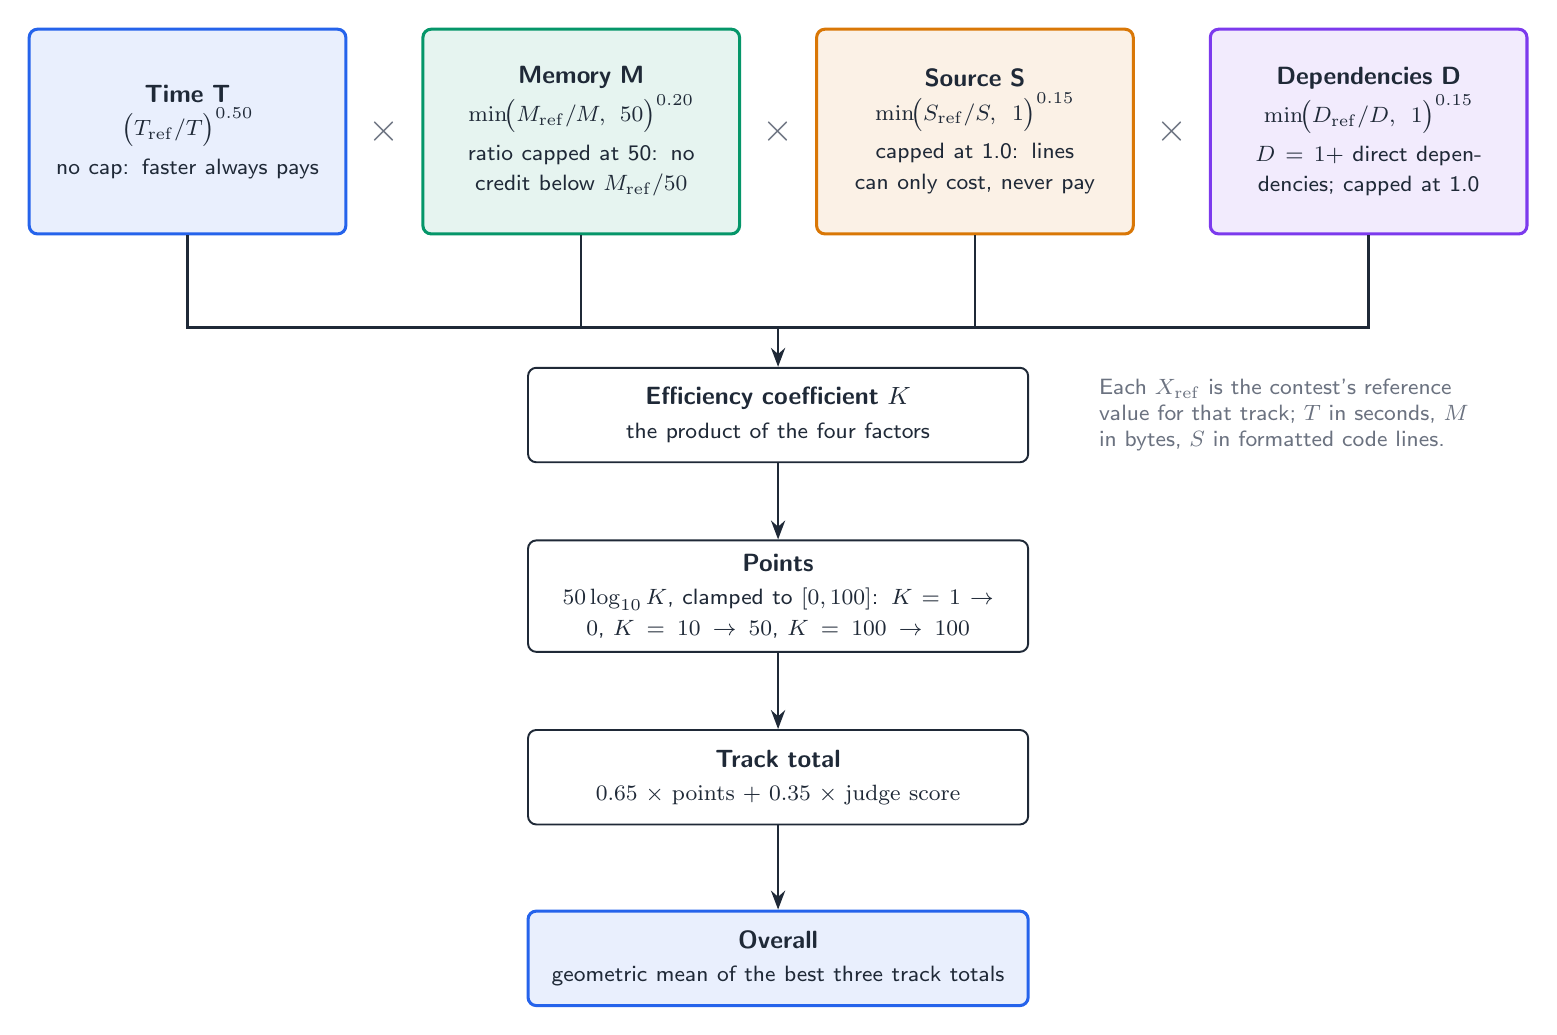
\begin{tikzpicture}
  \tikzset{term/.style={box=36mm, minimum height=26mm, inner sep=6pt}}
  \node[term, hl=cA] (t) at (0,0)    {\nt{Time T}{$\bigl(T_{\mathrm{ref}}/T\bigr)^{0.50}$}\par\vspace{3pt}{\footnotesize no cap: faster always pays}};
  \node[term, hl=cC] (m) at (5.0,0)  {\nt{Memory M}{$\min\!\bigl(M_{\mathrm{ref}}/M,\;50\bigr)^{0.20}$}\par\vspace{3pt}{\footnotesize ratio capped at 50: no credit below $M_{\mathrm{ref}}/50$}};
  \node[term, hl=cB] (s) at (10.0,0) {\nt{Source S}{$\min\!\bigl(S_{\mathrm{ref}}/S,\;1\bigr)^{0.15}$}\par\vspace{3pt}{\footnotesize capped at 1.0: lines can only cost, never pay}};
  \node[term, hl=cD] (d) at (15.0,0) {\nt{Dependencies D}{$\min\!\bigl(D_{\mathrm{ref}}/D,\;1\bigr)^{0.15}$}\par\vspace{3pt}{\footnotesize $D = 1 + $ direct dependencies; capped at 1.0}};

  \foreach \a/\b in {t/m, m/s, s/d}{
    \node[font=\Large, text=mute] at ($(\a)!0.5!(\b)$) {$\times$};
  }

  \node[box=60mm] (k) at (7.5,-3.6) {\nt{Efficiency coefficient $K$}{the product of the four factors}};
  \node[box=60mm] (p) at (7.5,-5.9) {\nt{Points}{$50\log_{10}K$, clamped to $[0,100]$: $K=1\to 0$, $K=10\to 50$, $K=100\to 100$}};
  \node[box=60mm] (tt) at (7.5,-8.2) {\nt{Track total}{$0.65\times\mathrm{points} + 0.35\times\mathrm{judge\ score}$}};
  \node[box=60mm, hl=cA] (o) at (7.5,-10.5) {\nt{Overall}{geometric mean of the best three track totals}};

  \foreach \x in {t,m,s,d}{
    \draw[ink, line width=0.9pt] (\x.south) |- ([yshift=5mm]k.north);
  }
  \draw[arr] ([yshift=5mm]k.north) -- (k.north);
  \draw[arr] (k) -- (p);
  \draw[arr] (p) -- (tt);
  \draw[arr] (tt) -- (o);
  \node[lab, anchor=west, text width=52mm] at (11.5,-3.6) {Each $X_{\mathrm{ref}}$ is the contest's reference value for that track; $T$ in seconds, $M$ in bytes, $S$ in formatted code lines.};
\end{tikzpicture}
\end{document}
